\documentclass[handout]{beamer}

% Lignes réponses
\usepackage{pgffor} % pour la commande \foreach permettant de réaliser une boucle
\newcommand{\pointilles}{{\\\rule{0pt}{1pt}\dotfill\rule{0pt}{1pt}}}
\newcommand{\rep}[1]{\foreach \n in {1,...,#1} {\pointilles}}

% Commandes pour cacher/révéler du texte facilement à l'aide d'un booléen
\usepackage{xstring}
\usepackage{ifthen}

\newboolean{reveal}
\setboolean{reveal}{false}

\newlength{\stextwidth} % une nouvelle longueur

\newcommand\x{6}

\newcommand{\guess}[1]{\ifthenelse{\boolean{reveal}}{{\color{red}#1}}{\settowidth{\stextwidth}{#1}\makebox[\stextwidth]{\dotfill}}}

\newcommand{\guessmath}[1]{\ifthenelse{\boolean{reveal}}{\textcolor{red}{#1}}{\settowidth{\stextwidth}{$#1$}\makebox[1.9\stextwidth]{\dotfill}}}

\newcommand{\guessmathbin}[1]{\ifthenelse{\boolean{reveal}}{\mathbin{\color{red}#1}}{\settowidth{\stextwidth}{$#1$}\makebox[2\stextwidth]{\dotfill}}}

% ========================================================================%

\usetheme{focus}

\usepackage{pgfpages}
\pgfpagesuselayout{4 on 1}[a4paper,landscape]

\usepackage[french]{babel}

\usepackage{xcolor}

\usepackage{pstricks,pst-plot,pst-text,pst-tree,pst-eps,pst-fill,pst-node,pst-math}
\usepackage{pstricks-add,pst-xkey}

\input ../tabvar

\usepackage{multicol}
\usepackage[np]{numprint}

\usepackage{minted}

\begin{document}

\title{}

\date{}

\begin{frame}
  \frametitle{Calculer avec des identités remarquables}
  Quels que soient les réels $a$ et $b$ :

  \[(a+b)^2 = \guessmath{a^2+2ab+b^2}\]

  \[(a-b)^2 = \guessmath{a^2-2ab+b^2}\]

  \[(a+b)(a-b) = \guessmath{a^2-b^2}\]

  \bigskip

  \textit{Remarque. -- Il faut savoir utiliser les identités précédentes dans les deux sens, c'est-à-dire pour développer et factoriser.}
\end{frame}

\begin{frame}
  Lorsque $a$ et $b$ sont positifs, l'identité remarquable 

  \[(a+b)^2 = a^2 + 2ab + b^2\]

  peut s'illustrer de la façon suivante :

  % dessin à faire ici
  \vspace{5cm}
\end{frame}

\begin{frame}
  \textit{Exemples. -- 
    \begin{enumerate}
      \item Développer puis réduire les expressions suivantes :
	\begin{multicols}{3}
	  \begin{itemize}
	    \item[(a)] $(2x+4)^2$
	    \item[(b)] $(x-7)^2$
	    \item[(c)] $(10x+2)(10x-2)$
	    \end{itemize}	
	\end{multicols}
      \item Factoriser les expressions suivantes :
	\begin{multicols}{3}
	  \begin{itemize}
	    \item[(a)] $y^2-10y+25$
	    \item[(b)] $4x^2-36$
	    \item[(c)] $4c^2+16c+16$
	  \end{itemize}
	\end{multicols}
	\item Python permet de développer des expressions :
	  \medskip
	  \begin{center}
	    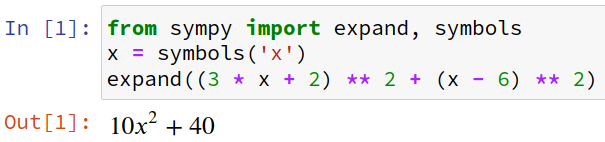
\includegraphics[width=10cm]{2_3_developper_avec_sympy.png}
	  \end{center}
    \end{enumerate}
  }
\end{frame}

\begin{frame}
  \textit{Exemple. -- $AEFD$ est un rectangle \og{}formé\fg{} d'un carré $ABCD$ de côté $x$ (avec $x>0$) et d'un rectangle $BEFC$ tel que $BE=2$. On note $\mathcal{A}$ l'aire du rectangle $AEFD$.
    \begin{center}
      \newrgbcolor{zzttqq}{0.6 0.2 0.}
      \newrgbcolor{ffxfqq}{1. 0.4980392156862745 0.}
      \psset{xunit=0.7cm,yunit=0.7cm,algebraic=true,dimen=middle,dotstyle=o,dotsize=5pt 0,linewidth=2.pt,arrowsize=3pt 2,arrowinset=0.25}
      \begin{pspicture*}(0.,0.)(7.,5.)
	\psline[linewidth=1.pt](1.,1.)(4.,1.)
	\psline[linewidth=1.pt](4.,1.)(4.,4.)
	\psline[linewidth=1.pt](4.,4.)(1.,4.)
	\psline[linewidth=1.pt](1.,4.)(1.,1.)
	\psline[linewidth=1.pt](4.,1.)(6.,1.)
	\psline[linewidth=1.pt](6.,1.)(6.,4.)
	\psline[linewidth=1.pt](6.,4.)(4.,4.)
	\uput[d](1,1){$A$}
	\uput[d](4,1){$B$}
	\uput[d](6,1){$E$}
	\uput[u](1,4){$D$}
	\uput[u](4,4){$C$}
	\uput[u](6,4){$F$}
      \end{pspicture*}
    \end{center}
    \begin{enumerate}
      \item Exprimer $\mathcal{A}$ en fonction de $x$.
      \item Vérifier que $\mathcal{A}=(x+1)^2-1$.
    \end{enumerate}
  }
\end{frame}

\end{document}

%%% Local Variables:
%%% mode: latex
%%% TeX-master: t
%%% End:
